\chapter{Multiple Importance Sampling Compensation}
\label{ch:mis_compensation}
Previous techniques didn't utilize the full potential of MIS,
because they didn't have the optimal pdf to create samples that are distributes proportional
to the integrand of the rendering equation~\ref{eq:rendering_equation}.
Karl\'ik et al.~\cite{Karlik2019} recognized this potential and created a techniques they called MIS compensation,
which chooses one sampling technique and refines it in a way that the final sampling distribution matches the integrand closer.\\
As we can see in Figure~\ref{fig:pdf_comparison} when we use our pdfs regularly with the balance heuristic
the resulting pdf is too defensive as the high values are undersampled and the low values are oversampled.
The name for their techniques comes from the compensation for the averaging of the balance heuristic.
One resulting pdf of their approach can be seen in Figure~\ref{fig:optimized_setup}.

\begin{figure}[h]
    \centering
    \begin{subfigure}[b]{.3\textwidth}
        \centering
        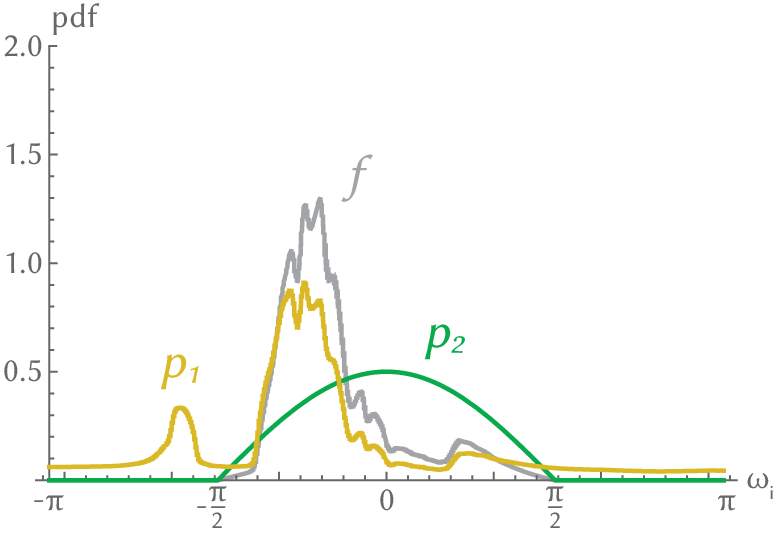
\includegraphics[width=\textwidth]{images/original_setup.png}
        \caption{Original pdfs}
        \label{fig:original_setup}
    \end{subfigure}
    ~
    \begin{subfigure}[b]{.3\textwidth}
        \centering
        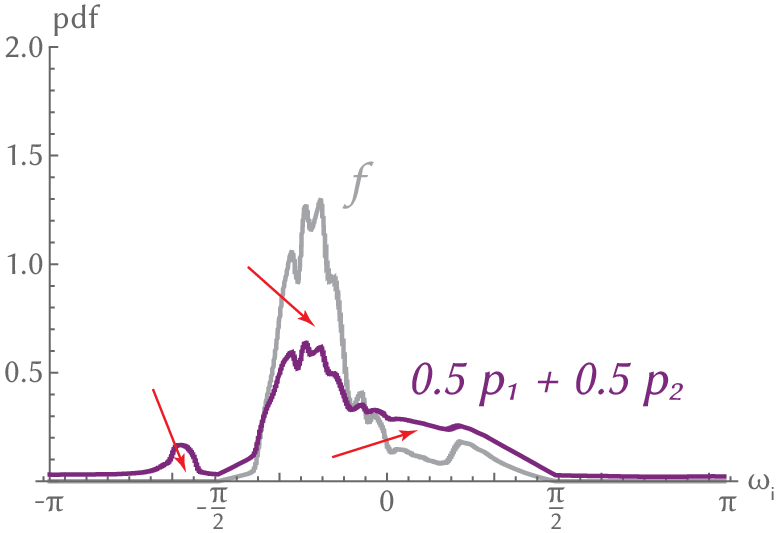
\includegraphics[width=\textwidth]{images/mis_setup.png}
        \caption{Original MIS}
        \label{fig:original_mis}
    \end{subfigure}
    \\
    \begin{subfigure}[b]{.3\textwidth}
        \centering
        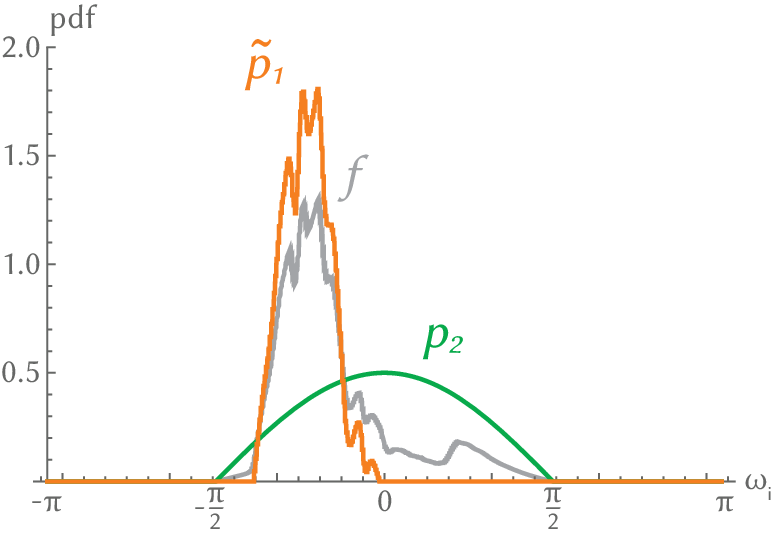
\includegraphics[width=\textwidth]{images/optimized_setup.png}
        \caption{Optimized pdfs
        \label{fig:optimized_setup}}
    \end{subfigure}
    ~
    \begin{subfigure}[b]{.3\textwidth}
        \centering
        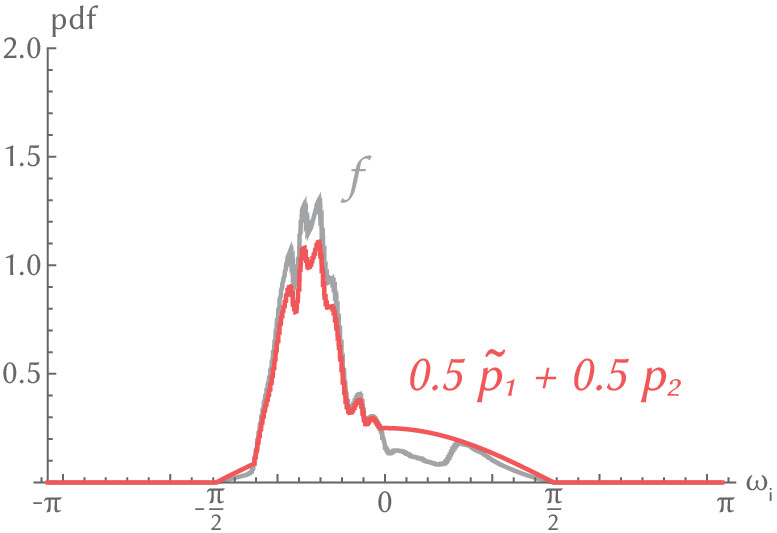
\includegraphics[width=\textwidth]{images/mis_optimized.png}
        \caption{Optimized MIS}
        \label{fig:optimized_mis}
    \end{subfigure}
    \caption{Comparison of the original pdfs without compensation~(\ref{fig:original_setup})
    and how the combined pdfs looks like with the balance heuristic~(\ref{fig:original_mis})
    and also the modified pdf~(\ref{fig:optimized_setup}) and the balance heuristic using the optimized pdf~(\ref{fig:optimized_mis}).
    $ f $ (gray) is the function we want to integrate.
    Figure~\ref{fig:original_mis} shows that the high values are undersampled and the low values are oversampled (see the red arrows).
    The optimized pdfs match the integrand much better when using MIS as seen in Figure~\ref{fig:optimized_mis}.
    \cite[Figure~2]{Karlik2019}}
    \label{fig:pdf_comparison}
\end{figure}

From a given set of samplers $ T $ they pick one sampler $ t \in T $ and call its pdf $ p_t $ the free pdf that will be used for compensation
so that the combined pdf reduces the variance when used with the balance heuristic.

In an optimal solution the combined pdf $ p_{eff}(x) = f(x)/F $ would lead to zero variance as shown in Equation~\ref{eq:zero_variance}.
For the purposes of MIS compensation the combined pdf can also be written as $ p_{eff}(x) = q(x) + c_t p_t(x) $ where $ q(x) = \sum_{i \in T/\{t\}} c_i p_i(x) $
and $ p_t $ is the free pdf with $ c_t $ being its fraction of the total number of samples.
We can reorder that to get a formula for
\begin{equation}
    \label{eq:compensated_pdf}
    p_t(x) = \frac{f(x)}{c_t F} - \frac{q(x)}{c_t}.
\end{equation}
This however does not guarantee that $ p_t $ is a valid pdf,
for this they clamped and normalized it and got this formula:
\begin{equation}
    \label{eq:valid_compensated_pdf}
    \tilde{p}_t(x) = \frac{1}{b} \max\{0, p_t(x)\}
\end{equation}
with a normalization factor of $ b = \int_X \max\{0, p_t(x)\} dx $.

Their compensated pdf fills the gap between the other samplers and the target function $ f(x) $
since it effectively samples only the parts that the other samplers missed in regard to $ f(x) $.
Whenever $ f(x) > 0 $ also $ p_{eff}(x) > 0 $ has to hold true for it to be unbiased.
When we assume $ q(x) = 0 $ then $ p_t(x) > 0 $, because of its definition~\ref{eq:compensated_pdf}.
If $ q(x) > 0 $ then $ p_t(x) $ could become $ 0 $, but then still $ p_{eff}(x) > 0 $ would be the case.
So the combined pdf is valid but it doesn't guarantee to reduce variance, because of the max operator and the re-normalization.


\section{Optimality}
\label{sec:misc_optimality}
Since the pdf from Equation~\ref{eq:valid_compensated_pdf} doesn't guarantee a variance reduction
we will take a look in this section at how a truly optimal pdf $ p_t^*(x) $ can be created for the free pdf.
First we look at the variance
which can be written as $ E(x^2) - E(x)^2 $ that equals in our case to $ J(p) - F^2 $ with $ J(p) = \int_X \frac{f(x)^2}{q(x) + c_t p(x)} $.
The optimal compensating pdf would then be $ p_t^*(x) = \underset{p}{arg~min}~J(p) $.
To make sure $ p_t^*(x) $ is a valid pdf we also set these two constraints $$ p_t^*(x) > 0 \text{, and } \int_X p_t^*(x) dx = 1 $$
In the original paper~\cite[Appendix~A]{Karlik2019} they used the Karush-Kuhn-Tucker constraints
to derive the optimal solution as $$ p_t^{\pm}(x) = \frac{f(x)}{\sqrt{c_t \lambda}} - \frac{q(x)}{c_t},~p_t^*(x) = \max\{0, p_t^{\pm}(x)\}. $$
$ \lambda $ is the Lagrange multiplier and ensures normalization.\\
Because of the max operator there is no analytical formulation for the solution and an iterative calculation is impractical in practice,
but if the MIS compensated solution from Equation~\ref{eq:valid_compensated_pdf} is close-enough to the optimal one it can be used instead.
The upcoming paragraphs will show that the compensated solution is indeed often similar to the optimal one.

\paragraph{Bounds for the MIS compensated solution}
To show the similarity of the optimal solution and the MIS compensated one
they derived the following bounds for $ \lambda $: $$ c_t F^2 \leq \lambda \leq \frac{1}{ct} F^2. $$
For a more detailed explanation of how they got the bounds please refer to~\cite[Appendix~B]{Karlik2019}.
From there we can then see that if $ p_t^{\pm}(x) > 0 $ then $ \lambda = c_t F^2 $ and with that $ p_t^*(x) = \tilde{p}_t(x) $.\\
In case they are not the same they checked how badly the compensated pdf could influence variance compared to the optimal one
and the worst case increase in variance is $ \frac{1}{c_t} $ as they proved in~\cite[Appendix~C]{Karlik2019}.
They also executed some tests to see how bad the compensated pdf could become in practice
and got a factor of $ 1.6 $ times the variance at most.

They showed that the compensated pdf is often equal to the optimal one
and in cases where it is not,
it's still a good solution,
since it can be easily obtained and doesn't introduce too much variance.